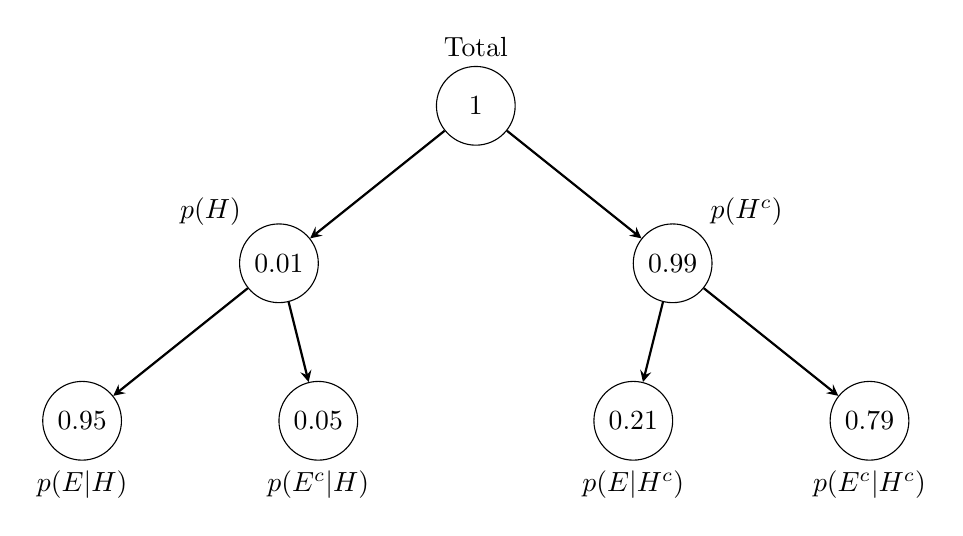
\begin{tikzpicture}
    \tikzstyle{arrow} = [thick,->,>=stealth]
    % Top bubble
    \node [draw, circle, minimum size=1cm, text centered, label={90:Total}] (Top) at (0,5) {1};

    % Lower left bubble
    \node [draw, circle, minimum size=1cm, text centered, label={135:$p(H)$}] (Diseased) at (-2.5,3) {0.01};
    \draw [arrow] (Top) -- (Diseased);

    % Lower right bubble
    \node [draw, circle, minimum size=1cm, text centered, label={45:$p(H^c)$}] (NonDiseased) at (2.5,3) {0.99};
    \draw [arrow] (Top) -- (NonDiseased);

    % Bottom extreme left
    \node [draw, circle, minimum size=1cm, text centered, label={-90:$p(E | H)$}] (TP) at (-5,1) {0.95};
    \draw [arrow] (Diseased) -- (TP);

    % Bottom mid left
    \node [draw, circle, minimum size=1cm, text centered, label={-90:$p(E^c | H)$}] (FN) at (-2,1) {0.05};
    \draw [arrow] (Diseased) -- (FN);

    % Bottom mid right
    \node [draw, circle, minimum size=1cm, text centered, label={-90:$p(E | H^c)$}] (FP) at (2,1) {0.21};
    \draw [arrow] (NonDiseased) -- (FP);

    % Bottom extreme right
    \node [draw, circle, minimum size=1cm, text centered, label={-90:$p(E^c | H^c)$}] (TN) at (5,1) {0.79};
    \draw [arrow] (NonDiseased) -- (TN);
\end{tikzpicture}

